\documentclass{article}
\usepackage[utf8]{inputenc}
\usepackage{graphicx}
\usepackage{hyperref}

\title{Research Methodology UE18CS400SG \\ Unit 2}
\author{Aditeya Baral}
\date{February 2022}

\begin{document}

\maketitle

\section{Research Design}

\begin{enumerate}
    \item Research Design is the preparation of the design of the research project 
    \item It constitutes the blueprint for the collection, measurement and analysis of data
    \item Revolves around questions like what the study is about, why is it being made, where will it be carried out, the type of data that will be required etc
\end{enumerate}

\subsection{Need for Research Design}

\begin{enumerate}
    \item Facilitate the smooth sailing of the various research operations
    \item Make research efficient (maximum information with minimal cost of money, effort, time)
    \item For collection and analysis of data that will be required
\end{enumerate}

Research Design stands for advance planning of methods to be adopted for relevant data collection and techniques used for their analysis keeping in view the objective of research and availability of staff, time and money

\subsection{Research Design Break Down}

\begin{enumerate}
    \item \textbf{Sampling Design} -- method to select items for study
    \item \textbf{Observational Design} -- conditions under which observations are made
    \item \textbf{Statistical Design} -- how many items to observe? how to gather and analyse data?
    \item \textbf{Operational Design} -- techniques of implementing steps in sampling, observational and statistical design
\end{enumerate}

\subsection{Concepts Related to Research Design}

\subsubsection{Dependent and Independent Variables}
A variable is a concept that can take on different quantitative values. Can be discrete or continuous.

A \textbf{dependent variable} depends on, or is a consequence of another variable. A variable \textit{antecedent} to the dependent variable is termed an \textbf{independent variable}.

\subsubsection{Extraneous Variable}

Extraneous variables are independent variables unrelated to the purpose of the study but may affect dependent variables. 

Any effect on a dependent variable due to an extraneous variable is termed an \textit{experimental error}. The term \textbf{control} is used to refer to restraining experimental conditions to minimise effects of extraneous variables.

\subsubsection{Confounded Relationship}

When the dependent variable is not free from the effect of extraneous variables, the relationship between the dependent and independent variables is said to be confounded by the extraneous variables.

\subsubsection{Research Hypothesis}

Testing of a prediction or hypothetical relationship using scientific methods.

It is a predictive statement relating one or more independent and dependent variables (must contain atleast one of each)

\subsubsection{Experiment and Non-Experimental Hypothesis Testing Research}

While testing the Research Hypothesis,
\begin{enumerate}
    \item \textbf{Experimental} -- independent variable is manipulated
    \begin{enumerate}
        \item Experiment under usual conditions -- \textbf{control group}
        \item Experiment under special conditions -- \textbf{experimental group}
    \end{enumerate}
    A study can include both control as well as both experimental groups.
    \item \textbf{Non-experimental} -- independent variable \textit{\textbf{not}} manipulated
\end{enumerate}

\subsubsection{Treatments}

The different conditions under which experimental and control groups are put are known as \textit{treatments}. Example, different types of techniques applied in a study are each considered a treatment.

\subsubsection{Experiment}

An \textit{experiment} is the examination of the truth of a statistical hypothesis related to a research problem. 

\begin{enumerate}
    \item \textbf{Absolute Experiment} -- determine impact or outcome of a study
    \item \textbf{Comparative Experiment} -- compare outcomes between studies
\end{enumerate}

\subsubsection{Experimental Units}

Pre-determined plots or blocks where different treatments are used are called \textit{experimental units}. These units must be selected and defined carefully.

\subsection{Basic Principles of Experimental Design}

\textbf{Fisher's Principles} of Experimental Designs state the following

\begin{enumerate}
    \item \textbf{Principle of Replication} 
    \begin{itemize}
        \item Repeat experiment multiple times
        \item Each treatment is applied in many experimental units
        \item Increases statistical accuracy of experiment
    \end{itemize}
    \item \textbf{Principle of Randomization}
    \begin{itemize}
        \item Design or plan experiment such that variations by extraneous factors can be all combined as due to \textit{chance}
        \item Provides protection against extraneous factors by randomization
    \end{itemize}
    \item \textbf{Principle of Local Control} 
    \begin{itemize}
        \item Vary extraneous factor (or known source of variability) over a wide range such that variability due to it can be measured
        \item Allows elimination of variability due to extraneous factors from experimental error
        \item Two-way analysis of variance -- treatments, extraneous factors and experimental error
        \item Divide the field into \textit{num\_treatments} homogeneous parts (process known as \textit{blocking}) where each block contains fixed extraneous factors. Measure value to check contribution to total variability using two-way variance analysis and then eliminate variability from extraneous factors from experimental error.
    \end{itemize}
\end{enumerate}

\subsection{Experimental Design}

\textit{Experimental Design} refers to the framework or structure of an experiment.

\subsubsection{Informal Experimental Design}

\begin{enumerate}
    \item \textbf{Before-and-after without Control}
    \begin{itemize}
        \item Measure dependent variable, apply treatment, measure again
        \item $Treatment\ Effect = phenomenon\ level_{after} - phenomenon\ level_{before} $
    \end{itemize}
    \item \textbf{After-only with Control}
    \begin{itemize}
        \item Two groups -- \textit{test} and \textit{control} with treatment added to test group
        \item $Treatment\ Effect = phenomenon\ level_{test} - phenomenon\ level_{control} $
    \end{itemize}
    \item \textbf{Before-and-after with Control}
    \begin{itemize}
        \item Two groups -- \textit{test} and \textit{control} with treatment added to test group
        \item Measure dependent variable in both groups, apply treatment to test group, measure both groups again
        \item $Treatment\ Effect = (phenomenon\ level_{test, after} - phenomenon\ level_{test, before}) - (phenomenon\ level_{control, after} - phenomenon\ level_{control, before}) $
    \end{itemize}
\end{enumerate}

\textbf{Important} -- Time periods for measurement must remain constant.

\subsubsection{Formal Experimental Design}

\begin{enumerate}
    \item \textbf{Completely Randomized}
    \begin{itemize}
        \item Involves only principles of replication and randomization
        \item Two approaches
        \begin{enumerate}
            \item \textbf{Two-group Simple Randomized} -- sample from defined population and assign to experimental or control group (follows principle of randomization). \textbf{Disadvantage} -- extraneous factors are not controlled.
            \item \textbf{Random Replications} -- each treatment is replicated a number of times to reduce effect of extraneous factors. Two populations (for study and to conduct experiments), sample from each, randomly assign to multiple experimental and control groups.
        \end{enumerate}
    \end{itemize}
    
    \item \textbf{Randomized Block}
    \begin{itemize}
        \item All principles are applied
        \item Subjects divided into groups (called blocks), keep extraneous factor fixed in each block to measure contribution to total variability
        \item Each treatment appears same number of times in each block
        \item Analyse using two-way variance analysis (two-way ANOVA technique)
    \end{itemize}
    
    \item \textbf{Latin Square}
    \begin{itemize}
        \item Frequently used in agricultural research
        \item An $n\ x\ n$ table with $n$ symbols, each symbol referring to a treatment such that each symbol appears once per row and column
        \item Used to control variation in two different directors (or two factors)
        \item Assign treatments randomly to combinations of the two factors keeping each treatment's occurrence as per point 2.
        \item 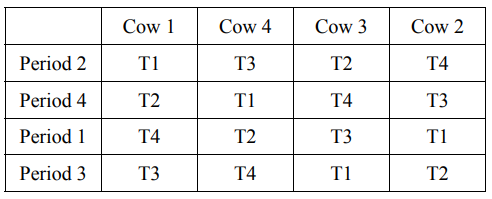
\includegraphics[width=0.7\linewidth]{img/LSD.png}
        \item \href{http://compneurosci.com/wiki/images/9/98/Latin_square_Method.pdf}{Refer section 1.1 and 2} 
    \end{itemize}
    
    \item \textbf{Factorial}
    \begin{itemize}
        \item Used to vary more than one factor  (independent variable) and find effect on dependent variable
        \item Mostly used for social and economic phenomena
        \item \begin{enumerate}
            \item Simple Factorial/Two-Factor Design -- 2 factors
            \item Complex Factorial/Multifactor Design -- $>$ 2 factors 
        \end{enumerate}
        \item If $n_{levels/treatments}^{(i)}$ corresponds to the number of levels or treatments for factor $i$, then the total number of cells in the design will be
        \begin{equation}
            {Number\ of\ cells\ in\ table} = \prod_{i=1}^{factors} n_{levels/treatments}^{(i)} 
        \end{equation}
    \end{itemize}
\end{enumerate}

\subsubsection{Features of a Good Research Design}
It must consider the following factors
\begin{enumerate}
    \item Means to obtain information
    \item Availability and skills of researchers
    \item Objective and nature of problem
    \item Availability of time and money for research
    \item Flexibility to consider different aspects
    \item Maximum accuracy with minimum bias
\end{enumerate}

\section{Sampling Design}

\begin{itemize}
    \item A \textbf{population} is a large group from which individuals are selected to participate in a study
    \item A \textbf{sample} is a smaller collection of individuals taken from a population for study. The sample must be representative of the \textbf{target population} from which the individuals were selected.
    \item Taking entire population in study is called \textbf{census} (\textit{impossible for cost reasons})
    \item A \textbf{sampling frame} is a list of all elements or other units containing the elements of a population
    \item Sample Design
    \begin{itemize}
        \item Plan for sampling
        \item Technique for selecting sample
        \item Sample design detected before and after sample collection
    \end{itemize}
\end{itemize}

\subsection{Steps in Sampling}
\begin{enumerate}
    \item \textbf{Objective} -- research objective in proportion with manpower, money and time
    \item \textbf{Population} -- clearly defined
    \item \textbf{Sampling Units and Frames} --  select unit for sample and sample source list
    \item \textbf{Sample Size} -- optimize for efficiency, flexibility, reliability
    \item \textbf{Parameters of Interest} -- statistical constants like mean
    \item \textbf{Data Collection} -- relevant information only
    \item \textbf{Non respondents} -- practical difficulties lead to data not being collected, changes results
    \item \textbf{Selecting Sampling Design} -- select technique that yields least error
    \item \textbf{Organize Field Work} -- reliable, trained personnel with supervisory staff
    \item \textbf{Pilot Survey} -- research on small scale before field scale
    \item \textbf{Budgetary Constraints} -- practical cost consideration, affects sampling decisions like size and technique
\end{enumerate}

\subsection{Sampling and Non-Sampling Errors}
\pagebreak

\begin{table}[htp]
\centering
\resizebox{\textwidth}{!}{%
\begin{tabular}{|l|l|}
\hline
\textbf{Sampling Error}                                                                                                                                        & \textbf{Non-Sampling Error}                                                                                  \\ \hline
\begin{tabular}[c]{@{}l@{}}Due to inferences made on \\ non-representative samples\end{tabular}                                                                & \begin{tabular}[c]{@{}l@{}}Due to improper data \\ collection and preparation\end{tabular}                   \\ \hline
Present only in sample                                                                                                                                         & Present in both census and sample                                                                            \\ \hline
\begin{tabular}[c]{@{}l@{}}Precision is measured for a sample size \\ and design, can be improved by  increasing \\ sampling size (but with cost)\end{tabular} & \begin{tabular}[c]{@{}l@{}}Reduced by defining sampling unit, \\ frame and population correctly\end{tabular} \\ \hline
\end{tabular}%
}
\end{table}

\subsection{Sampling Techniques}

\begin{enumerate}
    \item \textbf{Probabilistic} -- simple random, systematic, stratified, cluster
    \item \textbf{Non-Probabilistic} -- sequential, quota
\end{enumerate}

\subsubsection{Simple Random Sampling}
\begin{itemize}
    \item Probability based
    \item Randomly select without replacement
    \item Each individual has equal probability
    \item Becomes biased in large populations
\end{itemize}

\subsubsection{Systematic Sampling}
\begin{itemize}
    \item Randomly select start point, then select every $n^{th}$ individual
    \item List should not contain any hidden order
    \item Works well for large populations
\end{itemize}

\subsubsection{Stratified Sampling}
\begin{itemize}
    \item Performed when sample is not homogeneous, but possible to form homogeneous groups of population
    \item Divide population into homogeneous groups (called \textit{strata}) based on a factor that may influence dependent variable
    \item Perform \textit{simple random sampling} on each stratum
\end{itemize}

\subsubsection{Cluster Sampling}
\begin{itemize}
    \item Population divided into groups (if groups are geographic areas, called \textit{Area Sampling})
    \item Select samples from select groups
    \item \textbf{Advantages} -- useful when population is spread over large geographic area, convenient, reduced cost
    \item \textbf{Disadvantage} -- Less precise, representation issues likely
\end{itemize}

\subsubsection{Multistage Sampling}
\begin{itemize}
    \item More than 1 sampling technique used
    \item Complex and rarely used, requires more effort, time and cost
\end{itemize}

\subsubsection{Sequential Sampling}
\begin{itemize}
    \item Complex because size is not fixed
    \item Used for acceptance sampling
    \item A sequence of samples are taken from a lot
    \begin{itemize}
        \item When a particular lot to be accepted/rejected on basis of a single sample, it is called \textit{single sampling}. If two samples are used, it is called \textit{double sampling}. \textbf{If multiple but undefined samples are used, it is called sequential sampling}.
    \end{itemize}
\end{itemize}

\subsubsection{Quota Sampling}
\begin{itemize}
    \item Divide population into groups (like stratified)
    \item Judgement used to select individuals related to study from each group
\end{itemize}

\section{Data Collection}

\begin{enumerate}
    \item \textbf{Primary Data} -- data being collected for the first time, original, fresh, new
    \item \textbf{Secondary Data} -- data already collected before, been used for analysis
\end{enumerate}

\subsection{Collection of Primary Data}

\subsubsection{Observation}

\begin{itemize}
    \item Related to behavioral sciences
    \item Information without asking respondents
    \item Methods
    \begin{itemize}
        \item \textbf{Non-Scientific} -- observe surroundings
        \item \textbf{Scientific} -- plan and record, checks performed, validity tested
    \end{itemize}
    \item \textbf{Advantages} -- no subject bias, current happenings, independent of respondents
    \item \textbf{Disadvantages} -- expensive, limited information, unforeseen factors, people not always accessible
    \item \textbf{Terminologies}
    \begin{itemize}
        \item \textbf{Structured Observation} -- units, styles, standardised conditions, descriptive study
        \item \textbf{Unstructured Observation} -- exploratory study
        \item \textbf{Participant Observation}
        \item \textbf{Non-Participant/Disguised Observation}
        \item \textbf{Controlled Observation}
        \item \textbf{Non-Controlled Observation}
    \end{itemize}
\end{itemize}

\subsubsection{Interview}

\begin{enumerate}
    \item \textbf{Personal Interview}
    \begin{enumerate}
        \item Direct face-to-face questions asked
        \item Types
        \begin{enumerate}
            \item \textbf{Direct} -- interview source and collect data
            \item \textbf{Indirect} -- interview 3rd party close to source or someone who has knowledge about the problem 
            \item \textbf{Structured} -- structured data collection, predetermined question set and fixed order
            \item \textbf{Unstructured} -- flexible, no predetermined question set or order, interviewer given freedom to add/remove questions
            \item \textbf{Focused}
            \item \textbf{Clinical}
            \item \textbf{Non-Directive}
        \end{enumerate}
        \item \textbf{Advantages} -- more information, greater flexibility, easily obtained, low non-respondents, choice of respondent, less misinterpretation of questions
        \item \textbf{Disadvantages} -- expensive, time consuming, respondents not always approachable, bias due to interview presence, selection and training of staff required
        \item \textbf{Prerequisites} -- selection and training of interviewer, honesty, technical competence, practical experience, should not deviate from instructions
    \end{enumerate}
    
    \item \textbf{Telephonic Interview}
    \begin{enumerate}
        \item Collect data over telephone
        \item Not widely used (industry survey mainly)
        \item \textbf{Advantages} -- flexible, fast, cheap, responses can be recorded, easy to call back, no field staff, higher number and wider range of respondents
        \item \textbf{Disadvantages} -- little time to answer, less geographic coverage, short questions and point answers, more bias of interviewer
    \end{enumerate}
\end{enumerate}

\subsubsection{Questionnaire}

\begin{enumerate}
    \item For economic and business surveys
    \item Conducted by private individuals, research workers, organizations, governments
    \item Fixed number and order of questions (open-ended, MCQ, T/F) to be filled out and returned
    \item \textbf{Advantages} -- low cost, large geographic area, no interviewer bias, larger response time, can contact non-approachable respondents, more responses leads to more accurate results
    \item \textbf{Disadvantages} -- low return rate, educated and cooperative respondents needed, no flexibility (cannot make changes to questionnaire once sent), slowest, may have incomplete or ambiguous responses
    \item \textbf{Pilot Study} needed to test questionnaire and make modifications based on study -- add, remove, reword, rephrase etc
\end{enumerate}

\subsubsection{Schedule}

\begin{enumerate}
    \item A \textit{schedule} is a set of questions (direct, open/close ended, tabular) which are asked by the interviewer (also called \textit{enumerator}), who also fills out the respondent's answers
    \item Schedules may be handed out to respondents to fill themselves
    \item Enumerators are appointed, help respondents fill out answers, explain objectives of study, clarify doubts
    \item \textbf{Advantages} -- useful for illiterate respondents, less non-respondents, reliable data
    \item \textbf{Disadvantages} -- expensive, requires selection and training of enumerators, enumerator bias, respondent not anonymous
\end{enumerate}

\pagebreak

\begin{table}[]
\centering
\resizebox{\textwidth}{!}{%
\begin{tabular}{|l|l|}
\hline
\textbf{Questionnaire}                        & \textbf{Schedules}                                \\ \hline
Respondent fills                              & Enumerator fills                                  \\ \hline
Cheap, economical                             & More expensive -- enumerators selection, training \\ \hline
Higher non-response                           & Lower non-response                                \\ \hline
Anonymous responses                           & Identity of respondent is known                   \\ \hline
Wider range of respondents                    & Smaller range covered by enumerators              \\ \hline
No personal contact                           & Needs personal contact                            \\ \hline
Required literate and cooperative respondents & Respondents may be illiterate                     \\ \hline
Depends on respondent answers                 & Depends on honesty of enumerator                  \\ \hline
\end{tabular}%
}
\end{table}

\subsection{Collection of Secondary Data}

Data already collected and analysed by someone else, available publicly for others to use.

\subsubsection{Published Secondary Data}

Publications from government bodies, journals, reports from organizations and academia, books, magazines, newspapers, websites, public records and historical documents.

\subsubsection{Unpublished Secondary Data}

Diaries, letters, biographies made available publicly

\subsubsection{Checklist for Secondary Data Collection}

\begin{enumerate}
    \item \textbf{Reliability} -- who collected, sources, methods used, time period
    \item \textbf{Suitability} -- data must suit the study
    \item \textbf{Adequacy} -- data must be adequate for study
\end{enumerate}

\subsection{Survey vs Experiment}

\begin{table}[htp]
\centering
\resizebox{\textwidth}{!}{%
\begin{tabular}{|l|l|}
\hline
\textbf{Survey}                                                                                        & \textbf{Experiment}                                                                        \\ \hline
Descriptive Research                                                                                   & Experimental Research                                                                      \\ \hline
Large data size                                                                                        & Small data size                                                                            \\ \hline
No manipulation                                                                                        & Deliberate manipulation                                                                    \\ \hline
\begin{tabular}[c]{@{}l@{}}Relationship between data and unknown\\ studied through survey\end{tabular} & \begin{tabular}[c]{@{}l@{}}Relationship between data and unknown\\ determined\end{tabular} \\ \hline
Casual analysis                                                                                        & Correlation analysis                                                                       \\ \hline
\end{tabular}%
}
\end{table}

\end{document}
